\chapter{Конструкторский раздел}
В данном разделе приводится описание общей структуры разрабатываемой системы, её основных модулей и структур данных. Подробно описываются методы и алгоритмы, выбранные для использования в системе.
\section{Структуры данных, используемых при нахождении размеров цилиндра}
Для нахождения геометрических размеров цилиндра использовались следующие структуры данных:

\begin{itemize}
	\item \texttt{Vector2.}
	Двухмерный вектор. Содержит в себе два атрибута, координаты \texttt{x} и \texttt{y}.
	
	\item \texttt{CylinderSize.}
	Размер цилиндра. Содержит в себе два атрибута, высоту \texttt{H} и радиус \texttt{R}.
	
	\item \texttt{Line.}
	Отрезок. Содержит в себе два атрибута, вектор \texttt{v1} и вектор v2.
	
	\item \texttt{Color.}
	Цвет. Содержит в себе три атрибута, соответствующие значения цветовых каналов \texttt{r, g, b}.
	
	\item \texttt{ImageBase.} 
	Базовый тип изображения, от него наследуются цветное изображение \texttt{ColorImage} и изображение в градациях серого \texttt{GrayscaleImage}.
	Содержит в себе массив значений пикселей изображения.
\end{itemize}
%
%\begin{figure}[H]
%	\centering
%	{
%		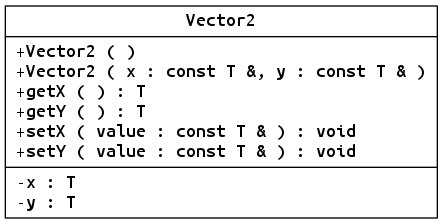
\includegraphics[scale=0.35,valign=t]{structs/Vector2.png}
%		\caption{}
%		\label{struct:types1}}
%\end{figure}
%\begin{figure}[H]
%	\centering
%	{
%		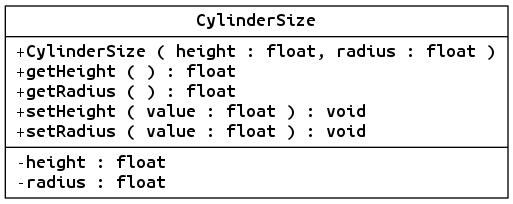
\includegraphics[scale=0.35,valign=t]{structs/CylinderSize.png}
%		\caption{Размеры цилиндра.}
%		\label{struct:types2}}
%\end{figure}
%\begin{figure}[H]
%	\centering
%	{
%		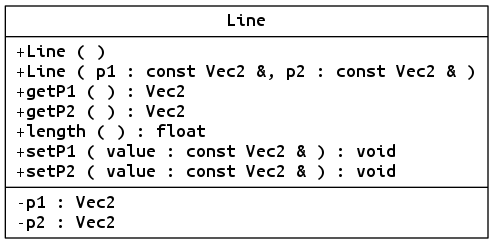
\includegraphics[scale=0.35,valign=t]{structs/Line.png}
%		\caption{Прямая.}
%		\label{struct:types3}}
%\end{figure}
%\begin{figure}[H]
%	\centering
%	{
%		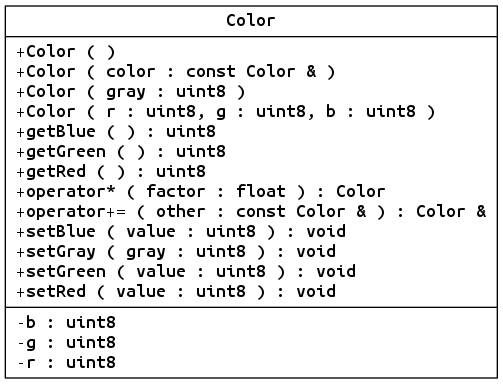
\includegraphics[scale=0.35,valign=t]{structs/Color.png}
%		\caption{Цвет.}
%		\label{struct:types4}}
%\end{figure}
%\begin{figure}[H]
%	\centering
%	{
%		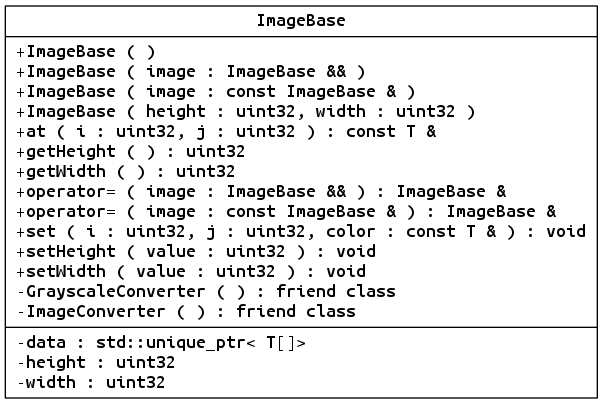
\includegraphics[scale=0.35,valign=t]{structs/ImageBase.png}
%		\caption{Базовый тип изображения, от него наследуются цветное изображение и изображение в градациях серого.}
%		\label{struct:types5}}
%\end{figure}

\section{Алгоритм нахождения размеров цилиндра}
Схема алгоритма нахождения размеров цилиндра представлена на рисунке \ref{fc:1}.
\begin{figure}[ht!]
	\centering{ 
		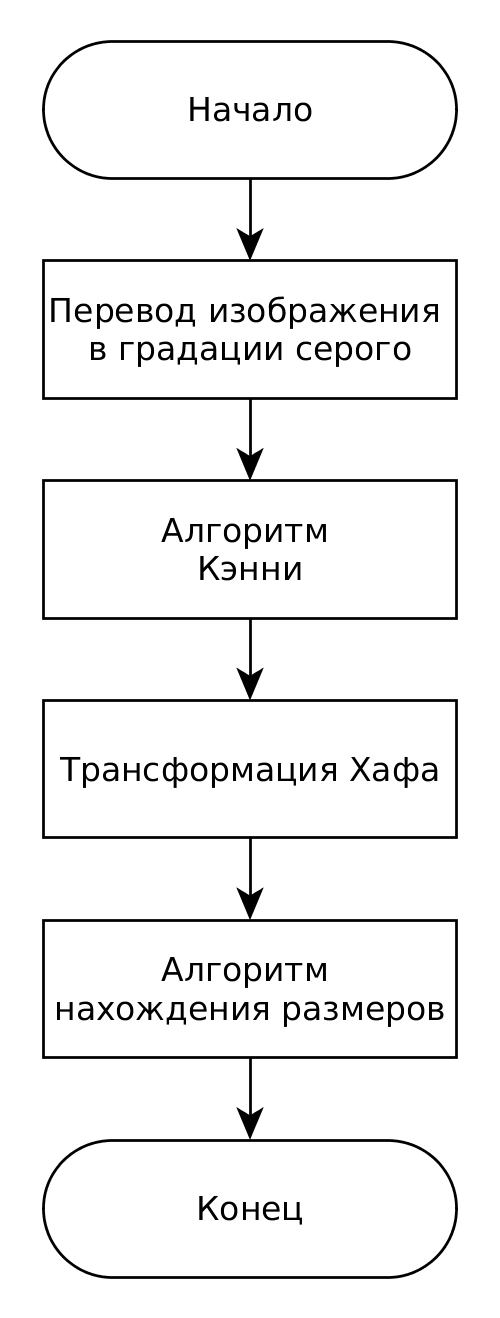
\includegraphics[width=0.32\textwidth]{img/fc1.png}
		\caption{Схема алгоритма нахождения размеров}
		\label{fc:1}}
\end{figure}




\section{Решение задачи определения геометрических размеров цилиндра}
При съемке цилиндра, с указанной позиции, диаметр цилиндра не виден полностью, а лишь его часть, как показано на рисунке \ref{an:vis}.

Зависимость размера видимой части цилиндра от высоты камеры \(CD = H\) и радиуса \(R\) можно вычислить согласно уравнениям (\eqref{eq:1}) - (\eqref{eq:2}).

\begin{gather}
\sin {\angle {ACO} } = \frac{AO}{CO} = \frac{R}{H-R} \label{eq:1} \\
\cos {\angle {ACO}} = \sqrt{1 - \sin ^2 {ACO}} = \sqrt {1 - (\frac {R}{H-R} )^ 2}\\ 
AE = R\cos {\angle {OAE}} = R\cos {\angle {ACO}} = R\sqrt {1 - (\frac {R}{H-R} )^ 2} \\
AB = 2AE = 2R\sqrt {1 - (\frac {R}{H-R} )^ 2} \label{eq:2}
\end{gather}

\begin{figure}[ht!]
	\centering{ 
		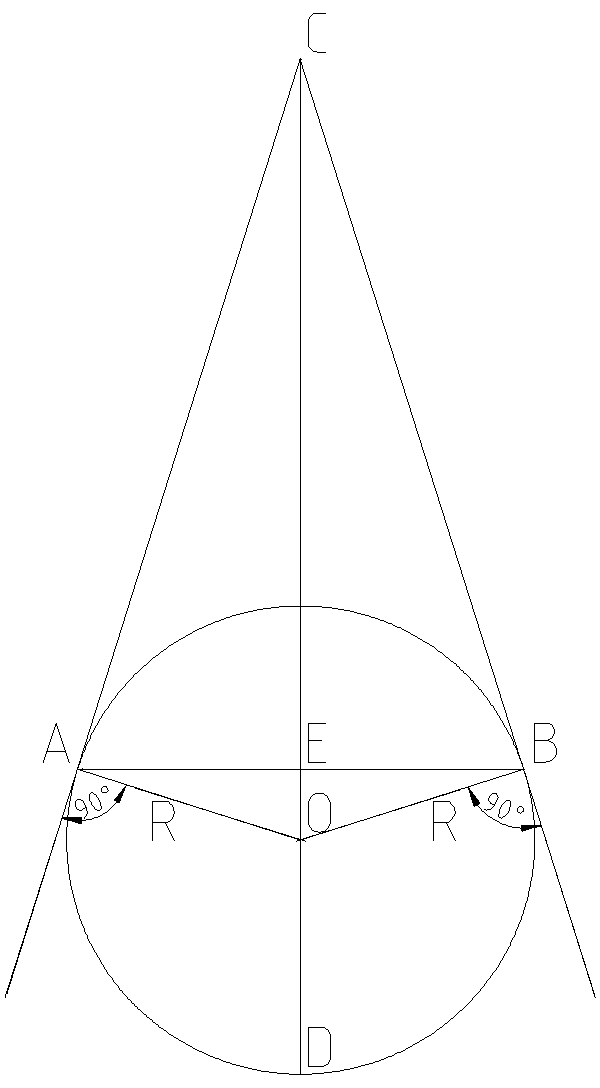
\includegraphics[width=0.3\textwidth]{img/analysis_1.png}
		\caption{Видимость цилиндра}
		\label{an:vis}}
\end{figure}

Длина \(AB\) будет соответствовать одному определенному значению радиуса \(R\) на промежутке \(I\), на котором длина \(AB\) возрастает. Верхнюю границу промежутка \(I\) можно найти из производной функции~\eqref{eq:1}.
Для случая, когда камера расположена на высоте \(H = 1\) метр, действителен следующий график:

\begin{figure}[ht!]
	\centering{ 
		\begin{tikzpicture}
		\begin{axis}[ 
		xmin=0,   xmax=1,
		ymin=0,   ymax=1,
		samples=401,
		xlabel=$R$,
		ylabel={$AB(R)$},
		] 
		\addplot [mark = none]{2*x*(1 - ( x/(1-x) )^ 2)^0.5 }; 
		\end{axis}
		\end{tikzpicture}
		\caption{Зависимость AB(R)}
		\label{an:vis1}
	}
\end{figure}

Из данной зависимости видно, что для корректной работы алгоритма, для данного случая, радиус цилиндра не должен превышать значение \(R=0.38197\) метра. В противном случае возникает неоднозначность.
Таким образом для промежутка \(I\) значение \(AB\) однозначно соответствует радиусу цилиндра и возможно однозначно определить высоту на которой находится \(AB\), и это значение можно использовать для вычисления масштабного коэффициента.

В вычислениях было сделано допущение, что лучи сходятся в одной точке. На самом же деле, лучи равномерно попадают на матрицу, которая имеет некоторые линейные размеры. Они были опушены, для упрощения вычислений и настройки программы.

\section{Структуры данных, используемых для трехмерного моделирования}
Для нахождения геометрических размеров цилиндра использовались следующие структуры данных:

\begin{itemize}
	\item \texttt{Vector3.}
	Трехмерный вектор. Содержит в себе 3 атрибута, компоненты x, y, z.
	
	\item \texttt{Scene.}
	Сцена хранит все объекты в динамическом массиве, которые можно на ней разместить: модель, камера, свет.
	
	\item \texttt{SceneObject.}
	Абстрактный класс объекта сцены. От него наследуются модель \texttt{Model}, камера \texttt{Camera}, абстрактный класс света \texttt{Light}. Каждый из перечисленных классов содержит в себе атрибуты, необходимые для его корректной работы.
	
	\item \texttt{Light.}
	Абстрактный класс света. От него наследуются модель рассеянный свет \texttt{AmbientLight}, точечный источник света \texttt{PointLight}.
	
	\item \texttt{Vertex.}
	Вершина. Состоит из координат, и нормали в данной позиции.
	
	\item \texttt{Mesh.}
	Меш  — набор вершин и многоугольников, определяющих форму трёхмерного объекта.
	Состоит из динамического массива вершин, и динамического массива треугольников \texttt{Triangle}. Треугольник содержит в себе три индекса вершин из массива меша.
	
	\item \texttt{Transformation.}
	Абстрактный класс преобразования объекта сцены. От него наследуются перемещение объекта сцены \texttt{MoveTransformation}, масштабирование -- \texttt{scaleTransformation}, поворот вокруг соответствующих осей -- \texttt{RotateXTransformation}, \texttt{RotateYTransformation}, \texttt{RotateZTransformation}, произвольное преобразование \texttt{CommonTransformation}, задаваемое матрицей \texttt{Mat4}. Классы содержат в себе матрицу преобразование и точку, относительно которой необходимо совершить преобразование.
	
	\item \texttt{Renderer.}
	Абстрактный класс преобразования объекта сцены. От него происходит рендер z-буффера со светом \texttt{LightZBufferRenderer}.
\end{itemize}

%\begin{figure}[H]
%	\centering
%	{
%		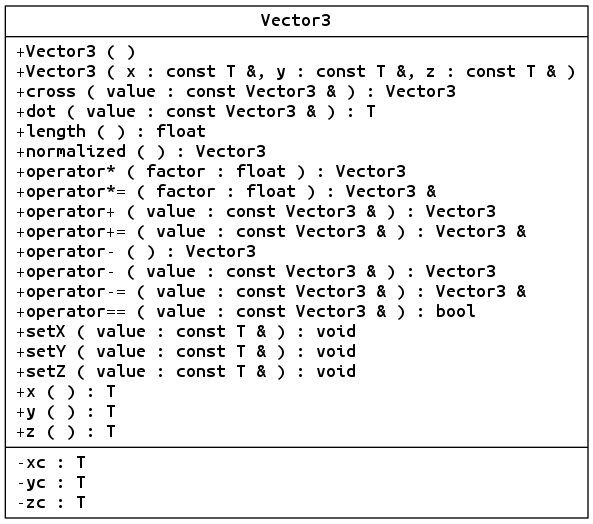
\includegraphics[scale=0.35,valign=t]{structs/Vector3.png}
%		\caption{Трехмерный вектор.}
%		\label{struct:types20}}
%\end{figure}
%\begin{figure}[H]
%	\centering
%	{
%		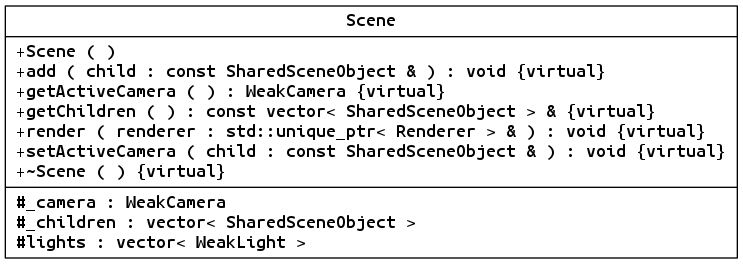
\includegraphics[scale=0.35,valign=t]{structs/Scene.png}
%		\caption{Сцена - хранит в себе все объекты, которые можно расположить на сцене: камера, модель, свет}
%		\label{struct:types22}}
%\end{figure}
%\begin{figure}[H]
%	\centering
%	{
%		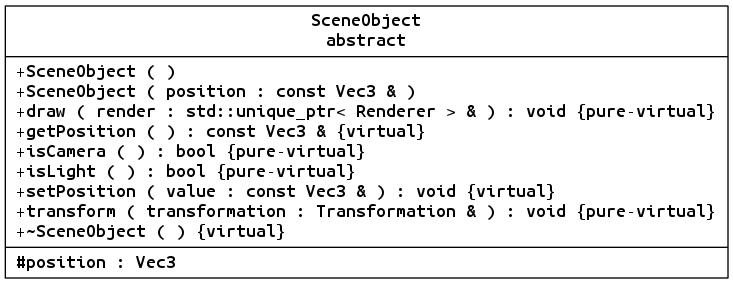
\includegraphics[scale=0.35,valign=t]{structs/SceneObject.png}
%		\caption{Абстрактный класс объекта сцены.}
%		\label{struct:types23}}
%\end{figure}
%\begin{figure}[H]
%	\centering
%	{
%		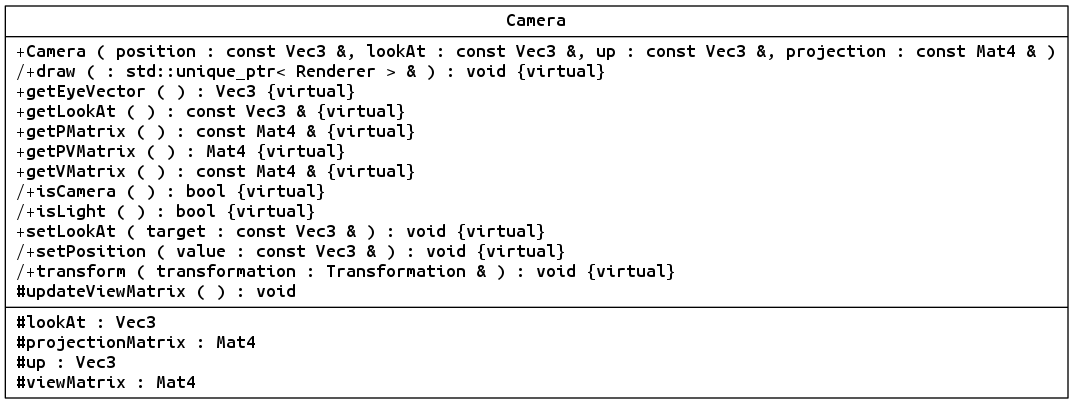
\includegraphics[scale=0.35,valign=t]{structs/Camera.png}
%		\caption{Абстрактный класс камеры.}
%		\label{struct:types24}}
%\end{figure}
%\begin{figure}[H]
%	\centering
%	{
%		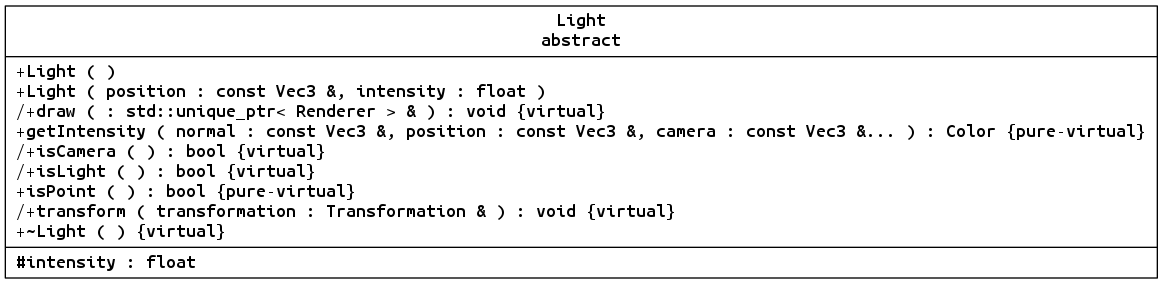
\includegraphics[scale=0.35,valign=t]{structs/Light.png}
%		\caption{Абстрактный класс света.}
%		\label{struct:types25}}
%\end{figure}
%\begin{figure}[H]
%	\centering
%	{
%		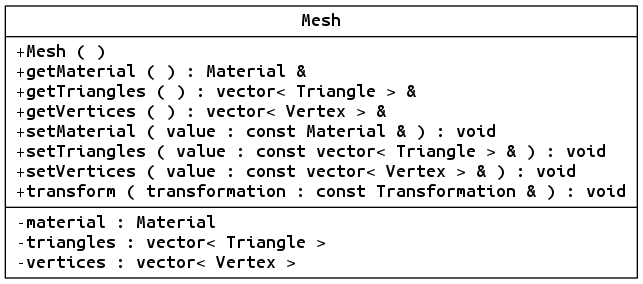
\includegraphics[scale=0.35,valign=t]{structs/Mesh.png}
%		\caption{Меш  — набор вершин и многоугольников, определяющих форму трёхмерного объекта.}
%		\label{struct:types26}}
%\end{figure}
%\begin{figure}[H]
%	\centering
%	{
%		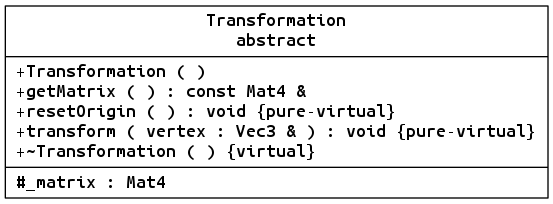
\includegraphics[scale=0.35,valign=t]{structs/Transformation.png}
%		\caption{Абстрактный класс преобразования объекта сцены.}
%		\label{struct:types27}}
%\end{figure}
%\begin{figure}[H]
%	\centering
%	{
%		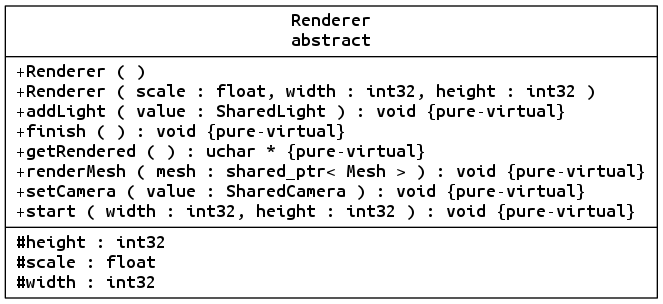
\includegraphics[scale=0.35,valign=t]{structs/Renderer.png}
%		\caption{Абстрактный класс рендера.}
%		\label{struct:types28}}
%\end{figure}


\section{Алгоритм рендеринга сцены}
Схема алгоритма рендеринга сцены представлена на рисунке \ref{fc:2}.
\begin{figure}[ht!]
	\centering{ 
		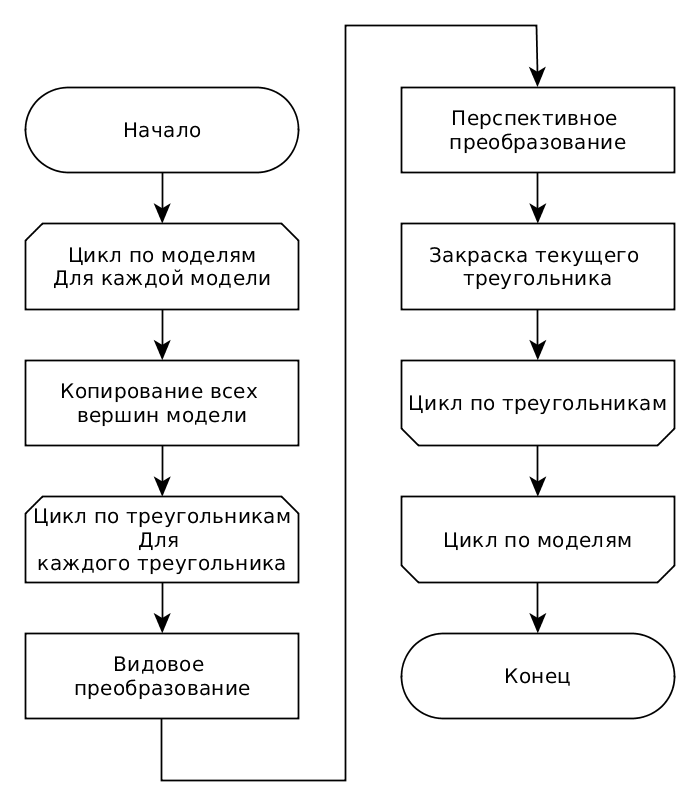
\includegraphics[width=0.68\textwidth]{img/fc2.png}
		\caption{Схема алгоритма рендеринга сцены.}
		\label{fc:2}}
\end{figure}
\section{Алгоритм закраски}
Схема алгоритма закраски треугольника представлена на рисунке \ref{fc:3.1}.
\begin{figure}[ht!]
	\centering{ 
		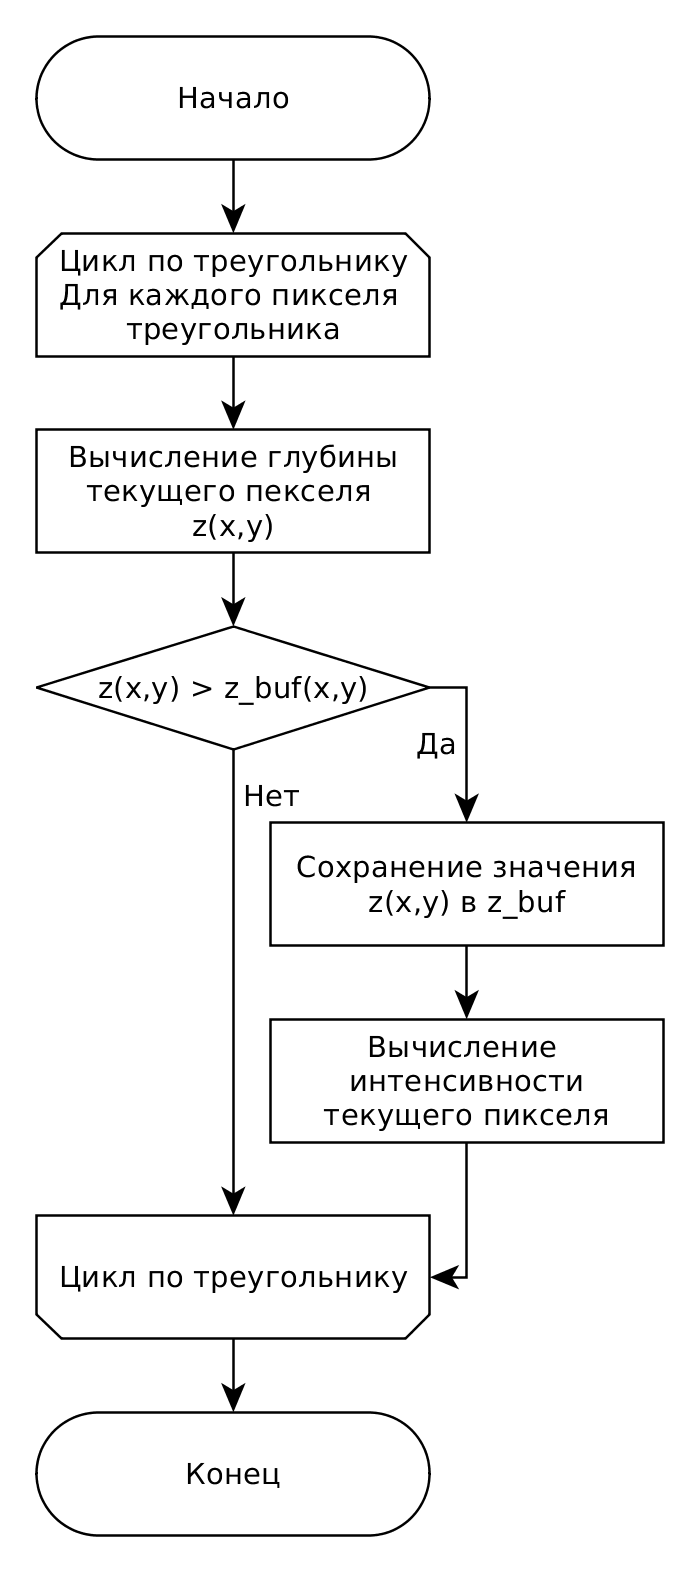
\includegraphics[width=0.5\textwidth]{img/fc3.png}
		\caption{Схема алгоритма закраски треугольника.}
		\label{fc:3.1}}
\end{figure}

